\documentclass{article}
\usepackage{lipsum}
\usepackage{graphicx}
\usepackage{wrapfig}

\begin{document}

\begin{figure}
    \centering
    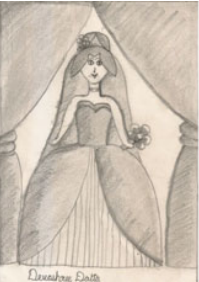
\includegraphics[width=2.0cm]{girl}
    \caption{A girl}
    \label{fig:girl}
\end{figure}


\begin{figure}
    \centering
    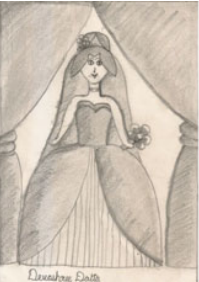
\includegraphics[width=2.0cm, angle=30]{girl}
    \caption{A girl}
    \label{fig:girl}
\end{figure}


\begin{figure}[!hbt]
    \centering
    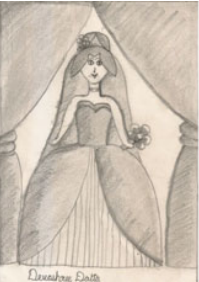
\includegraphics[width=2.0cm]{girl}\hfill
    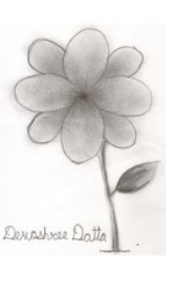
\includegraphics[width=2.0cm]{flower}
    \caption{A girl and a flower.}
    \label{girl_flower}
\end{figure}


\begin{figure}[!hbt]
    \begin{minipage}[c]{0.4\linewidth}
        \centering
        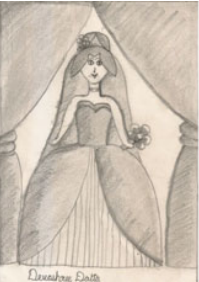
\includegraphics[width=3.0cm]{girl}
        \caption{A girl.}
        \label{girl}
    \end{minipage}\hfill
    %
    \begin{minipage}[c]{0.4\linewidth}
        \centering
        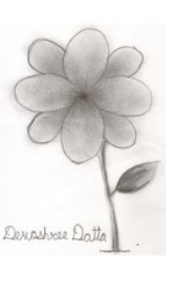
\includegraphics[width=2.5cm]{flower}
        \caption{A flower.}
        \label{flower}
    \end{minipage}
\end{figure}


\begin{figure}[!hbt]
    \begin{wrapfigure}[10]{r}{2.3cm}
        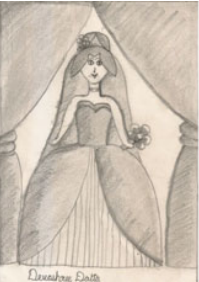
\includegraphics[width=2.0cm]{girl}
        \caption{Girl.}
        \label{girl}
    \end{wrapfigure}
    %
    \lipsum[1]
    $$x^2 + y^2 = z^2$$.
\end{figure}

\end{document}
